\section{Research and Counterfactual Workflow}
\label{sec:research-workflow}

GAWorld v2 treats an experiment as a configured execution that produces an
inspectable artifact tree, with each numeric result bound to a hash and an
evidence class.  The platform now exposes four research surfaces on top of
the underlying simulation: a matched-event workflow inherited from v1; a
parallel-worlds counterfactual engine; a Research Workbench that compiles a
paper or a research idea into a pre-registered protocol; and a
policy-simulation-and-optimization loop.  Each surface produces its own
artifact set and binds every result to the producing code path.  This
section describes the four surfaces; the Agent Playground and Arena are
covered separately in \cref{sec:playground-arena}.

\begin{figure}[t]
  \centering
  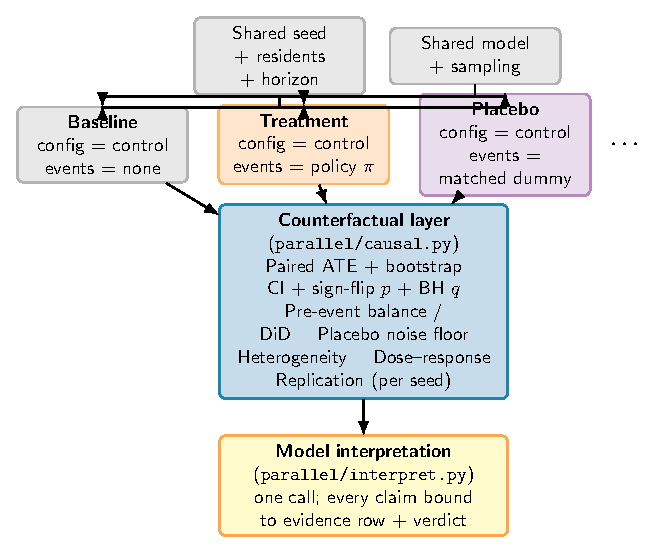
\includegraphics[width=\linewidth]{parallel_worlds.pdf}
  \caption{Parallel-worlds engine.  Up to eight matched worlds share the
  same seed, the same resident sample, and the same model.  Each world
  receives a per-world \texttt{config} patch and a per-world event list;
  the counterfactual layer then computes paired ATE, sign-flip $p$,
  pre-event balance, placebo noise floor, heterogeneity, dose--response,
  and replication.  An optional one-call model interpretation binds
  every claim to a specific evidence row.}
  \label{fig:parallel-worlds}
\end{figure}

\begin{figure}[t]
  \centering
  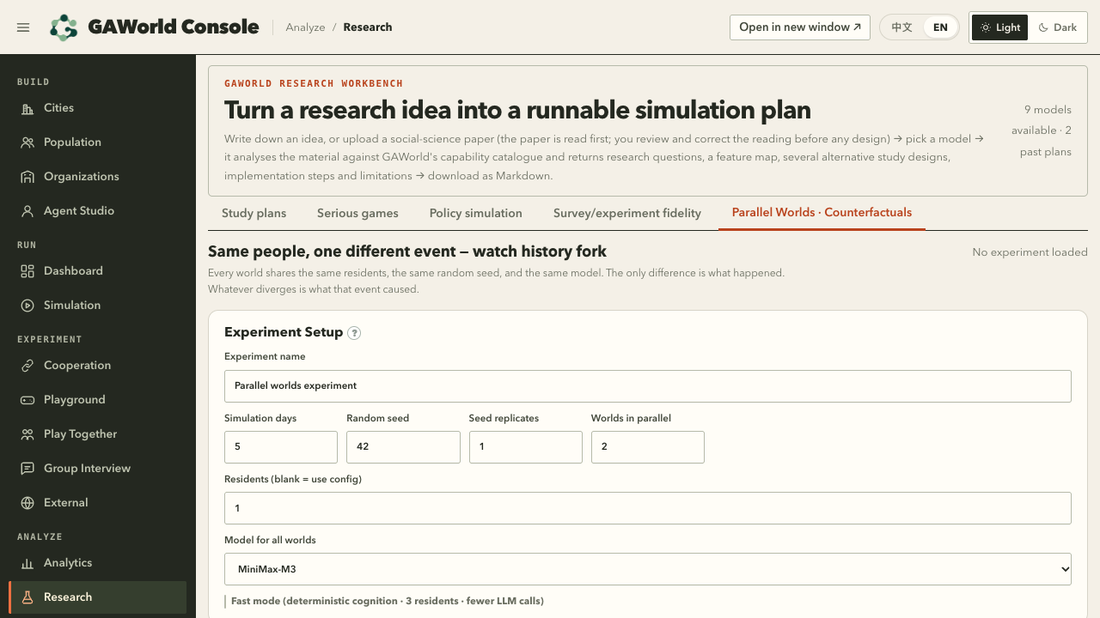
\includegraphics[width=\linewidth]{en_04_parallel.png}
  \caption{The Parallel Worlds tab.  A researcher fills in the experiment
  name, the simulation days, the random seed, the number of seed
  replicates (for the per-seed ATE and meta-analytic mean), the number of
  worlds to run in parallel (up to eight), the resident subset, and the
  model.  The \emph{Fast mode} toggle switches the engine to deterministic
  cognition with a smaller resident set so that the workflow can be
  rehearsed cheaply before a real run.}
  \label{fig:parallel-tab}
\end{figure}

\begin{figure}[t]
  \centering
  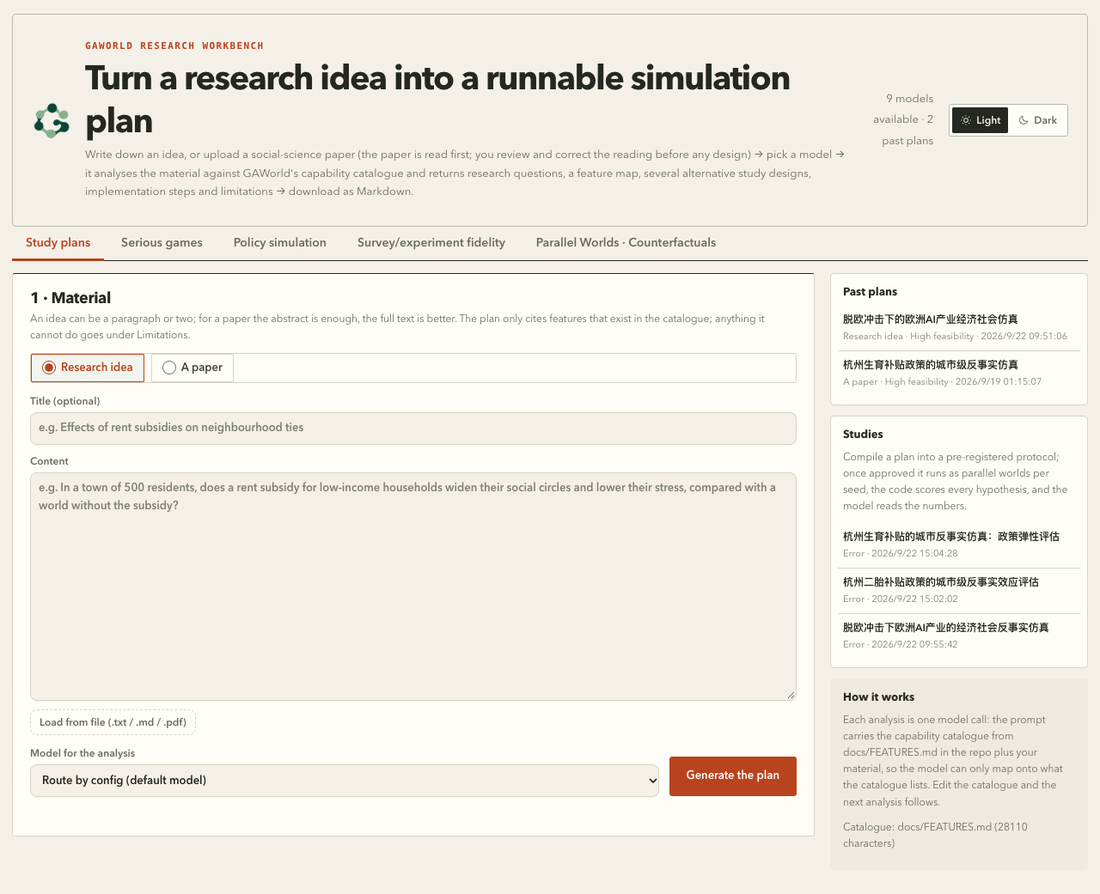
\includegraphics[width=\linewidth]{en_03_research.png}
  \caption{The Research Workbench.  A researcher pastes a research idea
  or uploads a paper, picks a model, and the system returns a plan: a
  theory, a methods paragraph, key variables, hypotheses, a feature map
  to the GAWorld surface, two or three experimental designs, and a list
  of limits.  The plan is editable; the model cannot write to a feature
  that is not in \texttt{FEATURES.md}, and the protocol compiler cannot
  use a metric that is not in the \emph{measurable catalog}.  The
  \emph{Study plans}, \emph{Serious games}, \emph{Policy simulation},
  \emph{Survey / experiment fidelity}, and \emph{Parallel Worlds
  Counterfactuals} tabs reuse the same pane to compile plans, run
  serious-game sessions, and run paper-fidelity studies.}
  \label{fig:research-workbench}
\end{figure}

\begin{figure}[t]
  \centering
  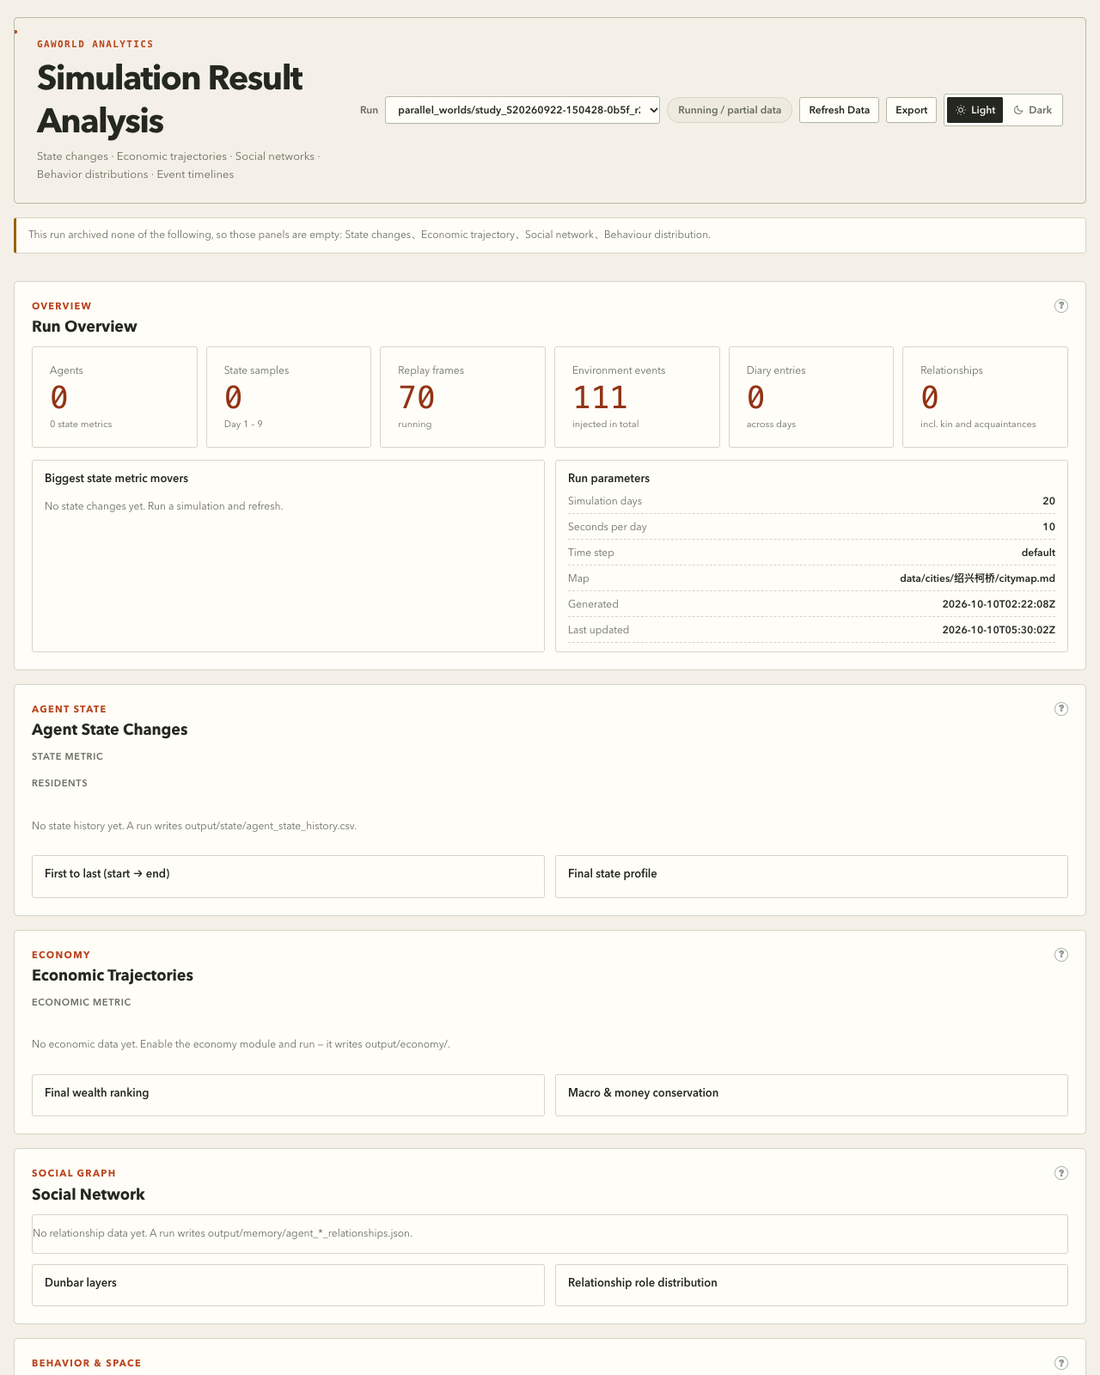
\includegraphics[width=\linewidth]{en_09_analytics.png}
  \caption{The Analytics pane.  After a run, the analytics pane exposes
  per-run counts (agents, state samples, replay frames, environment
  events, diary entries, relationships), a per-day event timeline broken
  down by source (\emph{social / natural / economic / political /
  life\_event / technology}), an event-type distribution, and an
  impact-tag distribution.  When a run is incomplete or a metric is
  missing, the pane displays \emph{No data yet} in the corresponding
  block rather than fabricating a value, in line with the evidence-class
  policy.}
  \label{fig:analytics}
\end{figure}

\subsection{Matched event and baseline runs}

For intervention studies, the \texttt{compare-event} command constructs two
scenario directories under a timestamped comparison root.  The
\texttt{without\_event} arm inherits the configured policy-event list, whereas
the \texttt{with\_event} arm appends a named event at an explicit simulation
day and clock time.  Both arms receive the same requested agent subset,
simulation horizon, random seed, and---when supplied---LLM provider override.
Before execution, each arm is reset within its own isolated memory, log,
vector-database, state, network, environment, intervention, and visualization
directories.  The two runs are then launched concurrently.  This organization
reduces accidental cross-arm state leakage and makes missing or failed arms
visible through separate reset and run logs.

After both subprocesses finish, the comparison routine reads each arm's
\texttt{state/agent\_state\_history.csv}.  For every available metric, it
computes the across-agent final snapshot, the mean over recorded observations,
and event-minus-baseline differences.  Machine-readable results are stored in
\texttt{comparison\_metrics.csv}; \texttt{comparison\_summary.md} provides a
human-readable view.  The separate \texttt{run\_meta.json} records choices
such as seed, horizon, provider, world identifier, node identifier, and
whether the lower-fidelity fast mode was requested.  v2 adds a
\texttt{warnings.json} that records any plugin or stage that failed to load
and the active plugin list; this makes the artifact self-describing about
which mechanisms were actually present.

\subsection{Parallel worlds and counterfactual inference}

The parallel-worlds engine generalizes the matched-event workflow.  An
\emph{experiment specification} describes up to eight worlds, a shared seed,
a per-world \texttt{config} patch, a per-world event list, and (optionally) a
set of replication seeds.  The engine runs the worlds sequentially under a
shared \texttt{GAWORLD\_CONFIG\_OVERRIDES} skeleton; the seed and the patch
together determine the per-world trajectory.  Per-arm completion status is
recorded in \texttt{worlds/<id>/run\_meta.json} and the per-arm artifact
trees are kept separate so that one arm's failure cannot contaminate another.

After all arms complete, the inference layer (\texttt{parallel/causal.py})
computes a deterministic counterfactual summary from the recorded state
trajectories.  No model call is made during inference.  The summary
includes:

\begin{itemize}[leftmargin=*]
  \item \textbf{Paired per-resident ATE} with a bootstrap confidence interval
  and a sign-flip $p$-value, for every metric that both arms recorded;
  \item \textbf{Pre-event balance} and a difference-in-differences estimator
  that uses the matched pre-event window as a baseline;
  \item \textbf{Placebo noise floor}: a separate placebo comparison that
  shows how large a difference arises from no intervention at all, with the
  same seed;
  \item \textbf{Onset order} and \textbf{heterogeneity}: the step at which
  the two trajectories first diverge and the per-resident effect size
  distribution;
  \item \textbf{Dose--response} for design points that vary an intervention
  parameter across worlds;
  \item \textbf{Replication} across seeds, with a per-seed ATE and a
  meta-analytic mean; and
  \item \textbf{Multiple-testing correction} with Benjamini--Hochberg
  $q$-values.
\end{itemize}

A study verdict is a function of the deterministic summary: a hypothesis is
\emph{supported} if its signed effect has $q<0.05$ and the replication mean
agrees in sign; \emph{reversed} if the sign agrees but the effect is
negligible; \emph{undetermined} if the replication is mixed; and
\emph{unmeasured} if the producing metric is missing in either arm.
The verdict gate is part of the same code path that the v1 GAWorld-Bench
used, so the meaning of a verdict is consistent across the two surfaces.

An optional one-call model interpretation (\texttt{parallel/interpret.py})
follows the inference.  The model sees the inference summary and the
per-comparison verdict and produces a brief narrative; every claim in the
narrative is bound to a specific evidence row and a verdict, and the
interpretation is cached per comparison so that reruns are deterministic
modulo provider noise.  v2 does not allow the model to overturn a
deterministic verdict: the verdict is the verdict.

\subsection{Research Workbench: from a paper or idea to a protocol}

The Research Workbench \citep{gaworldbench} divides a study into a planning
phase (output: a plan document) and an execution phase (output: a verdict
and a report).  The planning phase is a \emph{plan generator} that takes
either a research idea in free text or a paper (URL or PDF) and emits a
\emph{plan} with a theory, a methods paragraph, key variables, hypotheses,
a feature map to the GAWorld surface, two or three experimental designs,
an implementation outline, a credibility plan, and a list of limits.  The
plan is editable; the model cannot write to a feature that is not in
\texttt{FEATURES.md}, and the protocol compiler cannot use a metric that
is not in the \emph{measurable catalog}.

The execution phase is a \emph{protocol compiler} that takes the chosen
design and produces a \emph{pre-registered protocol}: a list of
conditions, a list of outcomes with pre-specified effect directions and
minimum effect sizes, a list of pre-registered exclusion rules, and a
list of confidence-thresholds.  A pre-execution check
(\texttt{research/evaluate.py}) verifies the protocol against the
measurable catalog and refuses to start a study that fails the check.
After the study runs, the deterministic verdicts are compared with the
pre-registered expectations; an \emph{unexpected} verdict is reported as
such and is not rewritten to look like the prediction.  The final
report contains the pre-registered protocol first, then the results,
then the interpretation, in that order.  This pattern follows the
spirit of the recent pre-registration literature in computational
social science and is intended to discourage post-hoc rewriting.

\subsection{Policy simulation and optimization}

The policy-simulation loop \citep{gaworldpolicy} takes a description of a
policy (and, optionally, a candidate version) and a fixed-scale sample of
residents, and produces a JSON reaction per resident.  The deterministic
scoring aggregator converts the residents' JSON into a composite score.
v2 then optionally calls a model with the score and the policy to propose
modifications; the modified policy is re-simulated on the same resident
sample, and the policy with the highest composite score is the
recommendation.  This is an \emph{optimization} in the sense that the loop
produces a candidate that scored higher than the original on the
deterministic composite; it is not a guarantee that the higher score
reflects a better real-world policy.  The loop is bounded by a maximum
number of iterations and by a hard cap on the number of LLM calls; the
artifact records both budgets and the policies it produced.

\subsection{Serious games and workshop studies}

The \emph{serious-game} module \citep{gaworldseriousgame} is a turn-based
role-play surface in which two or more roles are seated by a resident
agent or a human through a seat link.  Each round, the seated participants
respond simultaneously; a facilitator call resolves the round; a debrief
scores each role on a fixed rubric.  Designs and sessions are stored under
\texttt{output/research/serious\_games/} and re-loadable for inspection.
The serious-game surface is intended for participatory studies in which
the researcher wants to see how a human participant negotiates with
simulated residents under a fixed scenario; it is not a high-throughput
evaluation surface and is not used for benchmark scoring.

\subsection{Group interviews and persona distillation}

A \emph{group interview} is a one-shot elicitation across a roster of
residents, run as a child process per city and aggregated in the dashboard
\citep{gaworldinterview}.  Each resident answers a fixed set of questions
and the result is written to \texttt{output/interviews/<session\_id>/}
together with the resident's response, the producing code path, and the
model and seed that produced the answer.  A \emph{persona distillation}
takes a name or a URL and produces a sourced portrait (identity, state,
Big-Five, mental models, expression DNA, limits) that can be deployed as a
resident; the portrait and the producing research notes are stored under
\texttt{output/personas/<slug>/} and only \emph{deploy} writes the seed CSV
\citep{gaworldpersona}.  The deploy step is a separate, reviewed action
that the system refuses to perform automatically, so that an unverified
portrait cannot enter a population.

\subsection{What the workflow identifies}

The four surfaces above are useful scaffolds for counterfactual
experiments, but the recorded differences are still single contrasts
produced by an LLM-mediated dynamical system.  A common seed does not
guarantee common latent randomness after prompts diverge, and a policy
description does not guarantee that an economic or mobility mechanism
changed.  Before interpreting a difference, a researcher should verify
the intervention's path from event to structural state, replicate both
arms over seeds, pre-register target metrics, and include placebo events
or negative-control outcomes \citep{lipsitch2010negative}.  External
policy conclusions additionally require a defensible mapping to the
population and institutions of interest.  GAWorld v2 currently supports
constructing and auditing such a study, not replacing it.  The
deterministic verdict gate and the per-arm completion audit make a
defensible study easier to perform than the v1 system made it, but they
do not make a non-defensible study a defensible one.
